\documentclass[11pt]{article}
\usepackage[margin=1in]{geometry}
\usepackage{amsmath}
\usepackage{booktabs}
\usepackage{graphicx}
\usepackage{float}
\usepackage[hidelinks]{hyperref}
\emergencystretch=3em
\graphicspath{{figs/}}

\newcommand{\code}[1]{\texttt{#1}}

\title{The vibration at motor angle 120$^\circ$ in run 385\,psi, fan 800}
\author{Ilan Upfal}
\date{12 November 2026}

\begin{document}
\maketitle

\section*{Summary}

Run \code{DTU10MW\_385psi\_800fs} (9 October 2026) is the fastest run at
385\,psi: 6.9\,m/s, 32\,kg/m$^3$, $Re \approx 1.6\times10^5$. At motor angle
120$^\circ$ the blade vibrates harder than at any other angle in the sweep.
At this angle the arm points downstream, 30$^\circ$ off the flow direction.
The angle of attack is $+130^\circ$: the flow comes from the trailing-edge
side, with the chord at 50$^\circ$ to the flow. The inclination is
$+26^\circ$: the flow runs along the span from tip to root.
Section~\ref{sec:angles} gives the geometry.

\begin{enumerate}
  \item \textbf{It is the strongest vibration of the run.} The tip (S4) RMS
        is 2.9\,g edgewise and 4.3\,g flapwise, 3--5 times the median over all
        44 angles. Peaks reach 16.0\,g, right at the $\pm16$\,g range of the
        accelerometers, though no samples sit on the rail. The response is
        confined to about 110--130$^\circ$, the middle of region R1.
  \item \textbf{It is steady.} The amplitude holds for the whole 60\,s, with
        no bursts and no growth.
  \item \textbf{It is broadband forcing exciting the blade's resonances, not a
        clean single-frequency oscillation.} The whole spectrum rises 10--30
        times. The motion is irregular, and the main peaks carry only about a
        fifth of the variance.
  \item \textbf{Edgewise and flapwise move at different frequencies:}
        113\,Hz edgewise and a broad hump peaking at 143\,Hz flapwise. The
        edgewise frequency is the $\sim$110\,Hz peak this run shows at every
        angle. The flapwise one sits near the no-bolt 131/138\,Hz pair, and
        it changes with angle.
  \item \textbf{The whole blade bends.} The amplitude grows steadily from root
        to tip, and the root load cell sees the same 100--150\,Hz band
        rise about a hundredfold.
\end{enumerate}

%======================================================================
\section{Where 120$^\circ$ sits in the sweep}
%======================================================================

\begin{figure}[H]
  \centering
  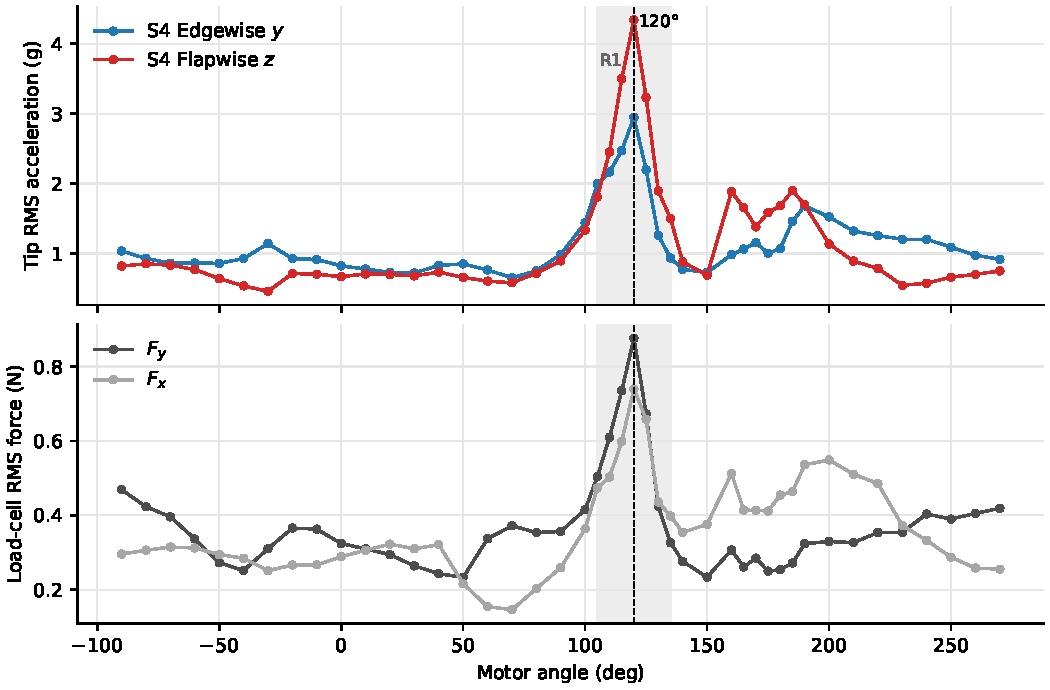
\includegraphics[width=0.9\textwidth]{sweep.pdf}
  \caption{RMS of the tip acceleration (top) and of the root load-cell
  forces (bottom) at each motor angle of the run. Grey band: region R1
  (105--135$^\circ$) of the PSD-analysis report. Dashed: 120$^\circ$.}
  \label{fig:sweep}
\end{figure}

Figure~\ref{fig:sweep} shows the whole sweep. Over most angles the tip RMS is
about 1\,g in each axis. Between 105 and 130$^\circ$ it rises to a sharp peak
at 120$^\circ$: 2.95\,g in $y$ and 4.34\,g in $z$. That is 3.0 and 5.4 times
the run's median, and 4.5 and 7.5 times the quietest angle (70$^\circ$). The
peak is narrow. By 135$^\circ$ the RMS is back to about 1--2\,g, and by
140$^\circ$ it is back to the baseline. The root load cell shows the same
peak: $F_y$ RMS is 0.88\,N, against a median of 0.34\,N.

Flapwise exceeds edgewise only around this peak and in the second, weaker
region near 160--190$^\circ$ (R2). Everywhere else the blade moves more
edgewise.

%======================================================================
\section{What the motion looks like}
%======================================================================

\begin{figure}[H]
  \centering
  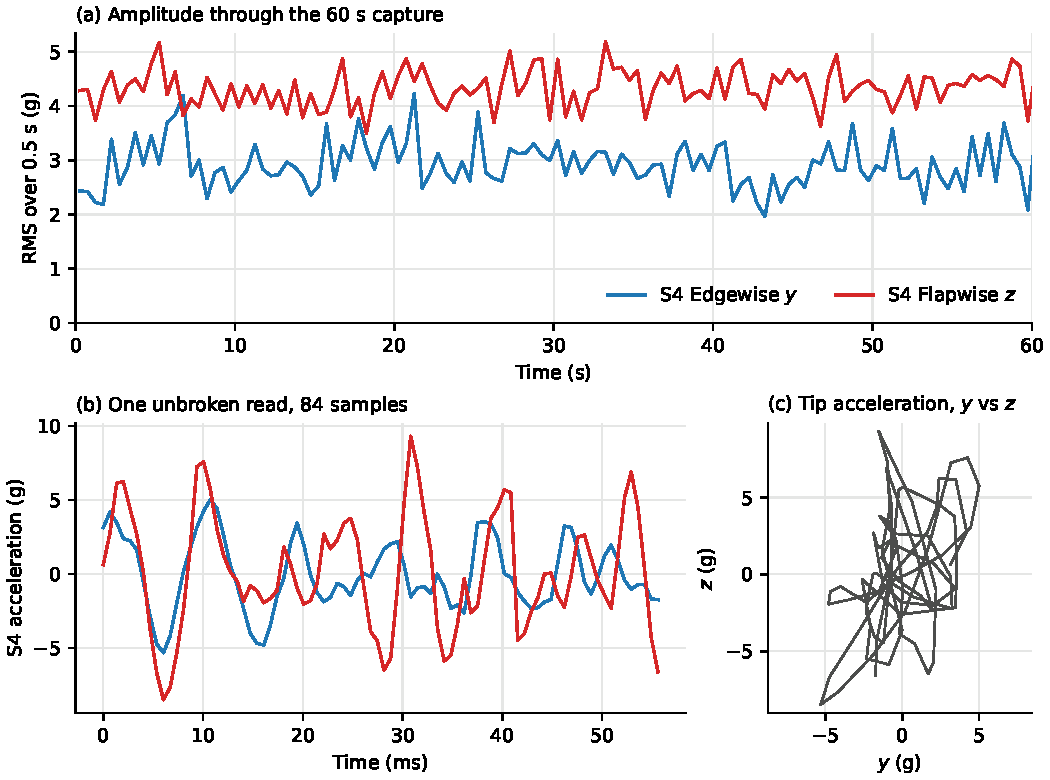
\includegraphics[width=0.9\textwidth]{time.pdf}
  \caption{Tip acceleration at 120$^\circ$. (a) RMS in 0.5\,s windows over
  the capture. (b) One read of 84 unbroken samples (56\,ms) from the middle of
  the capture. (c) The same 56\,ms of tip acceleration, $z$ against $y$ (not a displacement path).}
  \label{fig:time}
\end{figure}

\paragraph{Steady in time.} In Figure~\ref{fig:time}a the 0.5\,s RMS
fluctuates around a constant level: 2.0--4.2\,g in $y$ and 3.5--5.2\,g in $z$.
It neither grows nor dies away, and nothing switches on and off. A
spectrogram (Figure~\ref{fig:spectrogram}) shows the frequencies are steady
too. In 2\,s windows the edgewise peak stays at 102--118\,Hz (median 114) and
the flapwise peak at 130--153\,Hz (median 143).

\paragraph{Irregular in shape.} Panel~(b) is not a clean sine. Successive
cycles differ in height, and flapwise has large single swings of
$\pm$8--9\,g. The acceleration vector does not trace a repeating ellipse (panel~c) but
wanders. A self-excited oscillation locked to one frequency, such as flutter
or vortex lock-in, would look much more regular than this.

%======================================================================
\section{Frequencies}
%======================================================================

\begin{figure}[H]
  \centering
  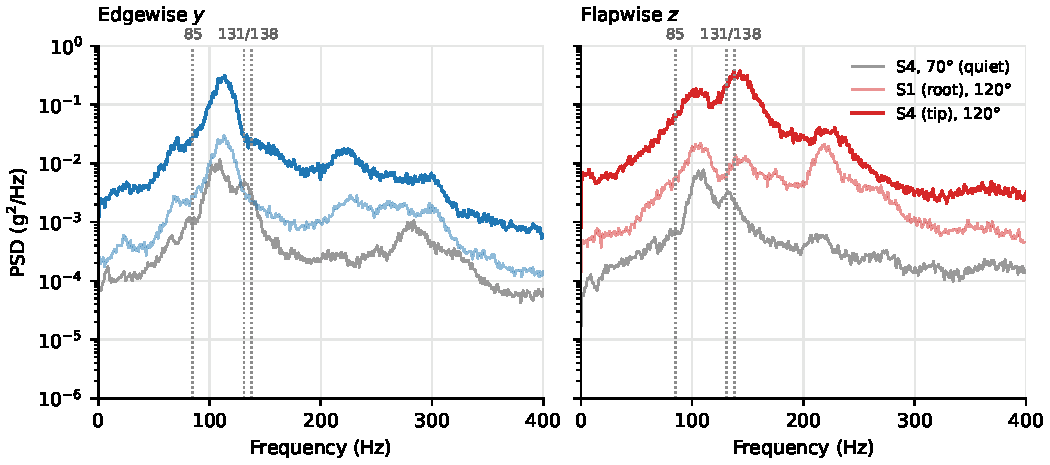
\includegraphics[width=\textwidth]{spectra.pdf}
  \caption{PSD at 120$^\circ$ at the tip (S4, dark) and root (S1, light),
  with the tip at the quietest angle (70$^\circ$, grey) for reference. Dotted
  lines: ring-down peaks of the blade without the mount bolt (85\,Hz mount;
  131/138\,Hz first-edge/second-flap pair). Welch, 2048-point segments
  (0.73\,Hz) on the 1493\,Hz sample grid, with the dropped samples masked.}
  \label{fig:spectra}
\end{figure}

Figure~\ref{fig:spectra} compares 120$^\circ$ with the quiet angle.

\begin{itemize}
  \item \textbf{The whole spectrum rises}, not just one peak. From 0 to
        400\,Hz the tip PSD at 120$^\circ$ is 10--30 times the quiet one, in
        both axes. Narrow bands around the main peaks hold only 22\% of the
        edgewise variance (113$\pm$4\,Hz) and 19\% of the flapwise variance
        (143$\pm$6\,Hz). The rest is spread across the band. So the flow at
        this angle forces the blade over a wide band, and the blade answers
        most strongly at its resonances.
  \item \textbf{Edgewise: a single peak at 113\,Hz.} The same peak is at
        108.6\,Hz at 70$^\circ$, about 30 times weaker. As the ring-down report
        notes, every angle of the fast runs shows this $\sim$110\,Hz peak. It
        matches no ring-down mode exactly.
  \item \textbf{Flapwise: a broad hump at 100--160\,Hz, peaking at 143\,Hz.}
        This is close to the no-bolt 131/138\,Hz pair (first edge and second
        flap) and to the bolted first edge mode (146\,Hz). The run summary
        gives 137.8\,Hz for the same peak; on a hump this broad, the exact
        maximum depends on the smoothing.
  \item \textbf{A weaker hump at 220\,Hz} appears in both axes, about twice
        113\,Hz. It is most likely a harmonic or a sum of the two main
        frequencies (113 + 107\,Hz), not a separate mode.
\end{itemize}

\paragraph{The two axes move largely independently.} At the tip, the
coherence between $y$ and $z$ is 0.44 at 113\,Hz and only 0.17 at 143\,Hz.
The flapwise motion at 143\,Hz is therefore not simply the edgewise mode seen
off-axis: the flow drives two separate responses. Nearer the root, the
flapwise spectrum also has a peak at 104--107\,Hz (Figure~\ref{fig:spectra},
light red), which is the coupled part.

\begin{figure}[H]
  \centering
  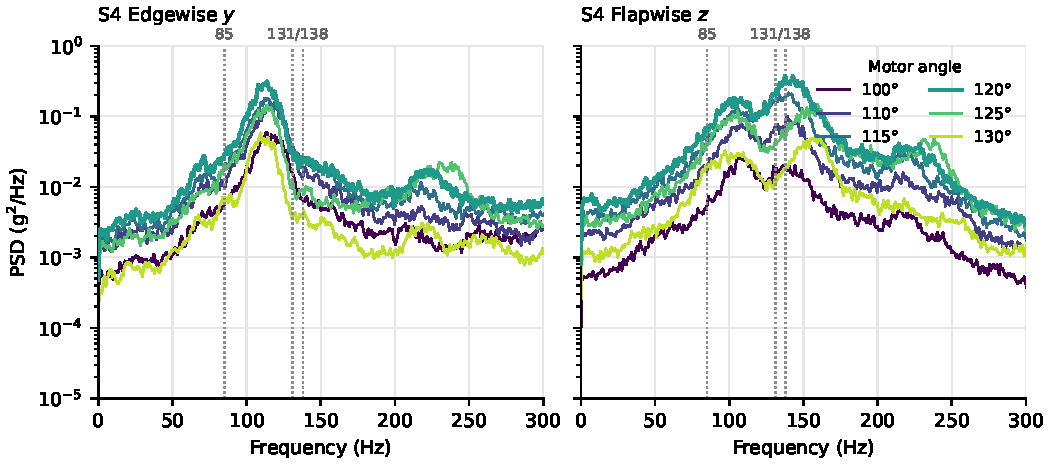
\includegraphics[width=\textwidth]{angles.pdf}
  \caption{Tip PSD at the angles around 120$^\circ$ (thick line).}
  \label{fig:angles}
\end{figure}

\paragraph{How the frequencies change with angle.} Figure~\ref{fig:angles}
shows the neighbouring angles. The edgewise peak hardly moves: from 100 to
140$^\circ$ it stays at 107--120\,Hz and only its height changes. The
flapwise peak jumps instead. Up to 105$^\circ$ it is at 104--109\,Hz,
together with the edgewise one. From 110 to 120$^\circ$ it is at
138--140\,Hz, and from 125 to 140$^\circ$ at 155--162\,Hz. So the strongest
vibration occurs where the flapwise response sits near 140\,Hz.

As a Strouhal number based on the mean chord (13.8\,mm), 113\,Hz is
$St = 0.23$ and 143\,Hz is $St = 0.29$. Across runs, the PSD-analysis report
found that R1 vibrates at fixed frequencies while the flow speed doubles,
which points to blade resonances rather than a frequency set by the flow.
This case fits that picture for the edgewise peak. The flapwise peak's
dependence on angle is not explained here.

%======================================================================
\section{Shape along the span and at the root}
%======================================================================

\begin{figure}[H]
  \centering
  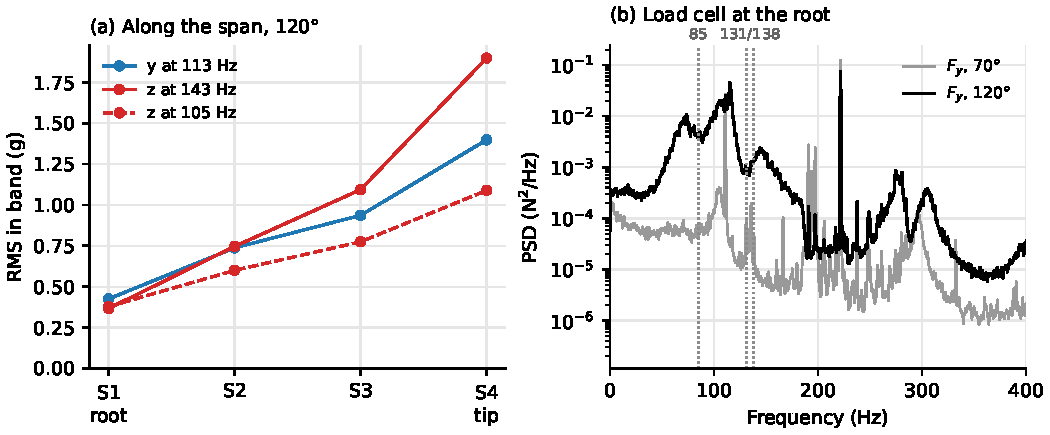
\includegraphics[width=\textwidth]{span_load.pdf}
  \caption{(a) RMS at 120$^\circ$ in narrow bands around each peak, at each
  sensor. (b) PSD of the root load cell's $F_y$ at 120$^\circ$ and at the
  quiet angle (70$^\circ$), sampled at 2\,kHz.}
  \label{fig:span}
\end{figure}

The amplitude grows smoothly from root to tip at every peak
(Figure~\ref{fig:span}a), as for a cantilever bending. The root-to-tip ratio
S1/S4 is 0.30 for edgewise at 113\,Hz and 0.19 for flapwise at 143\,Hz.
In the ring-down, the bolted blade modes gave 0.09--0.15 and the bolted
mount mode at 117\,Hz gave 0.36. Without the bolt, every mode gave about
0.25. The flapwise 0.19 is in the blade-mode range. The edgewise 0.30 at
113\,Hz is higher, between the no-bolt value and the mount mode, so the root
moves noticeably at this frequency. That fits the open question of whether
the 110\,Hz response at speed involves the mount. The blade still does most
of the bending.

At the root (Figure~\ref{fig:span}b), the load cell's $F_y$ PSD between
about 90 and 160\,Hz is roughly a hundred times its value at the quiet
angle, with the main peak at 110--115\,Hz. The sharp line at 222\,Hz is
equally strong at the quiet angle, so it does not come from this vibration.

%======================================================================
\section{Flow angles at 120$^\circ$}
\label{sec:angles}
%======================================================================

The angles come from the corrected transform
(\code{coordinate\_transforms.py}, 12 November 2026), which now also
writes \code{angle\_summary.csv}. The geometry follows the
experimentalists' sketch:
\begin{itemize}
  \item The motor turns the arm clockwise seen from above. At 0$^\circ$
        the arm points across the flow; at $+90^\circ$ it points
        downstream. At 120$^\circ$ it points downstream, 30$^\circ$ off
        the flow direction.
  \item The blade hangs from the arm tip, leaning 30$^\circ$ with its tip
        back toward the shaft.
  \item The chord is at the recorded mounting angle, 84.105$^\circ$, to the
        arm, with the leading edge upstream at motor 0$^\circ$.
\end{itemize}
The report \code{reports/angle\_check} gives the checks. Table~\ref{tab:angles}
lists the values.

\begin{table}[H]
  \centering
  \begin{tabular}{lcc}
    \toprule
    Source & Angle of attack & Inclination \\
    \midrule
    Corrected transform (= \code{master}), chord at 84.105$^\circ$ to arm & $+129.6^\circ$ & $+25.7^\circ$ \\
    Transform of 1 October (earlier \code{angle\_summary.csv}) & $-152.2^\circ$ & $-25.7^\circ$ \\
    \bottomrule
  \end{tabular}
  \caption{Flow angles at motor 120$^\circ$ (sweep $-30^\circ$). Angle of
  attack: from the chord (leading to trailing edge) to the flow.
  Inclination: positive when the flow runs from tip to root.}
  \label{tab:angles}
\end{table}

The 84.105$^\circ$ is $90^\circ - 5.895^\circ$ (\code{main.py}): the chord is
5.9$^\circ$ off perpendicular to the arm, so the angle of attack is
$+5.9^\circ$ at motor 0. An earlier draft of this report quoted the 1 October
transform's $-152^\circ$, which was wrong.

\paragraph{For a simulation of this case.} \code{reports/angle\_check/angle\_mapping.md}
gives the inflow direction in the blade's own axes, with check values. In
the beam model's frame (X toward the suction side, Y toward the trailing
edge, Z from root to tip), and with the reference chord along $+Y$, the
freestream direction is $(+0.695, -0.574, -0.433)$. The flow comes from the
pressure side, from trailing edge toward leading edge, and from tip toward
root.

%======================================================================
\section{Reading}
%======================================================================

At 120$^\circ$ the flow reaches the blade from the trailing-edge side
(angle of attack $+130^\circ$). The chord sits at 50$^\circ$ to the flow,
so the blade presents much of its width to it, and the flow also runs
along the span from tip to root (inclination $+26^\circ$). At such an angle
the flow is very probably separated,
and the forcing is broadband and unsteady. The blade responds at the
frequencies where it resonates: 113\,Hz edgewise and about 140\,Hz
flapwise. The response stays strong for as long as the blade is held at
this angle. Three things point to broadband (buffeting-type) excitation
rather than a self-excited oscillation such as flutter or vortex lock-in:
the raised spectrum everywhere, the irregular waveform, and the weak
coupling between $y$ and $z$.

Why 120$^\circ$ is so much worse than 110 or 130$^\circ$ is the open
question. One candidate is that the flow's forcing peaks at this angle.
Another is that the flapwise response near 140\,Hz lines up there with a
blade resonance; Figure~\ref{fig:angles} shows the flapwise peak passing
through 140\,Hz exactly in the 110--120$^\circ$ range. Spectra at finer
angle steps (every 1--2$^\circ$ from 110 to 130$^\circ$) would separate the
two.

\paragraph{Caveats.}
\begin{itemize}
  \item The tip $z$ reaches 15.98\,g, within 0.1\% of full scale. No sample
        is clipped, but a slightly larger response would saturate. The
        $\pm$16\,g range is already the largest the LIS2DS12 offers.
  \item About 16\% of the samples are lost between reads (the 84-on, 16-off
        pattern). This puts weak copies of each peak 14.4\,Hz away
        (about 3\% of the parent's PSD). They do not affect the peaks
        discussed here.
  \item The mode labels follow the ring-down report: the blade was most
        likely run without the mount bolt, and the 110\,Hz peak of the fast
        runs matches no ring-down mode exactly.
\end{itemize}

\appendix
\section{Spectrogram}

\begin{figure}[H]
  \centering
  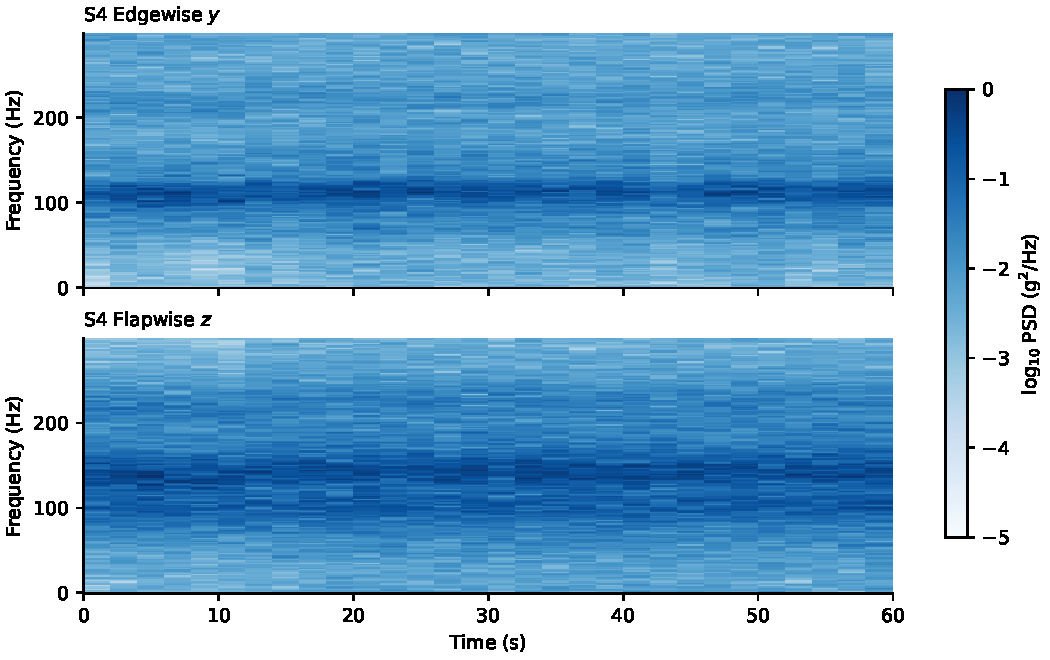
\includegraphics[width=0.9\textwidth]{spectrogram.pdf}
  \caption{Tip PSD in 2\,s windows (1024-point segments) through the 60\,s
  capture at 120$^\circ$.}
  \label{fig:spectrogram}
\end{figure}

Figures and numbers: \code{reports/case\_385psi\_800fs\_120deg/make\_figures.py}.

\end{document}
